
In the inclusive \BtoXsgamma analysis, the aim is to reconstruct an inclusive sample of all possible \Xs states, 
as described before (e.g. \Cref{sec:exp_overview}).
This means that explicit requirements on the momentum, number of tracks, angles etc. of the \Xs system may introduce a direct bias on the `inclusiveness' of the measurement.
Assessing the impact of selections on $X_s$ in a model-independent way is difficult.
Therefore, the \Xs system is treated in a completely `missing-momentum' approach, such that no direct requirements on it are imposed.
The reconstruction requirements are only applied on the candidate tag-side $B$ meson and the candidate high-energy photons from \BtoXsgamma.
\subsection{Tag-side \texorpdfstring{$B$}{B}-meson candidate reconstruction}

The analysis begins with a reconstruction of a $B$ meson candidate in each event using the Belle II Full Event Intepretation (\FEI) algorithm \cite{Keck:2017mui,Keck:2018lcd}.
\todo[inline]{Do I describe FEI here or in software section? not sure yet}

This thesis uses data and simulation samples following the standard Belle II approach, where sub-samples of data and \MC with FEI algorithm applied are produced centrally, referred to as \textit{\FEI skims}.
In order to make the \FEI algorithm run-time and computation more efficient, event selections are made which reject events highly incompatible with one of the $B$ mesons decaying hadronically.
This decision is based on tracks and clusters as per standard Belle II reconstruction guidelines with additional selections, summarised in \Cref{tab:fei_objects}.
In essence, they ensure that only energetic tracks originating from the interaction point are selected;
and to minimise the impact of beam-background clusters, or clusters where no track information can be associated (outside of CDC acceptance).

\begin{table}[htbp!]
    \centering
     \caption{\label{tab:fei_objects} Definitions for \FEI event pre-selection.}
     \resizebox{0.75\textwidth}{!}{
     \begin{tabular}{lcc} 
     Selection description & Selection\\
     \hline
     Cleaned tracks & $  |d_0|<0.5~\cm,\quad z_0<2~\cm,\quad p_T>0.1~\gev $\\
     Cleaned \ECL clusters & $17~\degrees<\theta<150~\degrees,\quad E>0.1~\gev$\\
     \end{tabular}
     }
\end{table}

Using the definitions of cleaned tracks and \ECL clusters, a requirement on each event is imposed, and only the events that pass these requirements are analysed by the \FEI algorithm.
The requirements are summarised in \Cref{tab:fei_precuts}.

\begin{table}[htbp!]
    \centering
     \caption{\label{tab:fei_precuts} \FEI pre-selections.}
     \resizebox{0.75\textwidth}{!}{
     \begin{tabular}{lcc} 
     Selection description & Selection\\
     \hline
     Number of cleaned tracks in event \quad & $\geq 3$\\
     Number of cleaned \ECL clusters in event \quad & $\geq 3$\\
     Total measured center-of-mass energy in the event \quad & $> 4~\gev$\\
     Total energy of cleaned \ECL clusters \quad &\multirow{2}{*}{$2~\gev<E<7~\gev$}\\
     and deposits associated with with cleaned track \quad & \\
    \end{tabular}
     }
\end{table}
The requirements to have at least 3 clean tracks in the event and at least 3 clean \ECL clusters is based on the fact, that a hadronic day will produce many charged tracks and photons.
Furthermore, measured energy in the event in the \epem collision center-of-mass frame is required to exceed 4~\gev.
This is a purely pragmatic requirement: based on the fact that no neutrinos or missing-momentum are present in a hadronic decay, the energy cannot be much lower than 5.28~\gev.
Finally, the total deposited energy registered by the \ECL in the event is required to lay between 2 and 7~\gev.
This requirement ensures that
\todo[inline]{ensures what tbh?}

The events that pass through requirements of \Cref{tab:fei_precuts} are further passed to be analysed by the \FEI algorithm.
In each event multiple \FEI candidates are reconstructed.
To focus only on the candidates that have been correctly reconstructed, selection on \DeltaE and \Mbc are made, as well as a loose-requirement on \feiProb.

\todo[inline]{explain that these cuts ar eok for photon energy}
\subsection{Candidate photon reconstruction}

As discussed, besides the tag-side reconstruction in $B$-hadronic modes, only the photon from \BtoXsgamma can be reconstructed while ensuring a model-independent inclusive measurement.
In order to reduce the quickly growing number of background-photon candidates, only events where there is at least photon with $\Estar>1.2~\gev$ are considered.
The photons must also be within the CDC acceptance ($17--150~\degrees$).
These requirements are summarised in \Cref{tab:photon_requirements}.
\begin{table}[htbp!]
    \centering
     \caption{\label{tab:photon_requirements} Requirements for photons in reconstructed events.}
     \resizebox{0.75\textwidth}{!}{
     \begin{tabular}{lcc} 
     Selection description & Selection\\
     \hline
     Number of photons with \Estar>1.2~\gev & $  N(\Estar>1.2~\gev)\geq1 $\\
     Polar angle of photon & $17~\degrees<\theta<150~\degrees$\\
     \end{tabular}
     }
\end{table}

Reconstructed photon energy is transformed, based on XXX.

\subsection{Overview of the selected sample}

After reconstruction, based on \MC samples, there can be up to 20 tag-$B$ candidates and up to 2 signal-photon candidates, although having 2 photon candidates is highly unlikely.
By ranking each candidate based on \EB and \feiProb, a two-dimensional grid of relative fraction of combinations of tag-$B$ candidates and photons is made.
This is shown in \Cref{tab:grid_photon_fei}.
The sample is broken down to show the relative fraction of total number of tag-side $B$ meson candidates in \Cref{fig:fei_tag_reco_candidates}.

\begin{table}[htbp!]
    \caption{\label{tab:grid_photon_fei} Grid.}
    \centering
\begin{minipage}[c]{0.395\textwidth}
    \centering
    Generic tag \Bp reconstruction
    \resizebox{1\textwidth}{!}{
        \begin{tabular}{lrrr}
            \hline
            gamma\_gammaE\_rank &   1.0 &   2.0 &   All \\
            Btag\_feiSigRank &       &       &       \\
            \hline
            1.0             & 0.483 & 0.001 & 0.484 \\
            2.0             & 0.235 & 0.001 & 0.236 \\
            3.0             & 0.118 & 0.000 & 0.118 \\
            4.0             & 0.066 & 0.000 & 0.066 \\
            5.0             & 0.037 & 0.000 & 0.038 \\
            6.0             & 0.022 & 0.000 & 0.022 \\
            7.0             & 0.013 & 0.000 & 0.013 \\
            8.0             & 0.009 & 0.000 & 0.009 \\
            9.0             & 0.005 & 0.000 & 0.005 \\
            10.0            & 0.003 & 0.000 & 0.003 \\
            11.0            & 0.002 & 0.000 & 0.002 \\
            12.0            & 0.001 & 0.000 & 0.001 \\
            13.0            & 0.001 & 0.000 & 0.001 \\
            14.0            & 0.001 & 0.000 & 0.001 \\
            15.0            & 0.000 & 0.000 & 0.000 \\
            16.0            & 0.000 & 0.000 & 0.000 \\
            17.0            & 0.000 & 0.000 & 0.000 \\
            18.0            & 0.000 & 0.000 & 0.000 \\
            All             & 0.997 & 0.003 & 1.000 \\
            \hline
            \end{tabular}  
    }
\end{minipage}
\begin{minipage}[c]{0.395\textwidth}
    \centering
    Generic tag \Bz reconstruction
    \resizebox{1\textwidth}{!}{
        \begin{tabular}{lrrr}
            \hline
            gamma\_gammaE\_rank &   1.0 &   2.0 &   All \\
            Btag\_feiSigRank &       &       &       \\
            \hline
            1.0             & 0.561 & 0.001 & 0.562 \\
            2.0             & 0.229 & 0.000 & 0.229 \\
            3.0             & 0.098 & 0.000 & 0.098 \\
            4.0             & 0.050 & 0.000 & 0.050 \\
            5.0             & 0.025 & 0.000 & 0.025 \\
            6.0             & 0.015 & 0.000 & 0.015 \\
            7.0             & 0.008 & 0.000 & 0.008 \\
            8.0             & 0.005 & 0.000 & 0.005 \\
            9.0             & 0.003 & 0.000 & 0.003 \\
            10.0            & 0.001 & 0.000 & 0.001 \\
            11.0            & 0.001 & 0.000 & 0.001 \\
            12.0            & 0.001 & 0.000 & 0.001 \\
            13.0            & 0.000 & 0.000 & 0.000 \\
            14.0            & 0.000 & 0.000 & 0.000 \\
            15.0            & 0.000 & 0.000 & 0.000 \\
            16.0            & 0.000 & 0.000 & 0.000 \\
            17.0            & 0.000 & 0.000 & 0.000 \\
            18.0            & 0.000 & 0.000 & 0.000 \\
            19.0            & 0.000 & 0.000 & 0.000 \\
            All             & 0.999 & 0.001 & 1.000 \\
            \hline
            \end{tabular}
            
            
    }
\end{minipage}
\end{table}

\begin{figure}[htbp!]
    \centering
    \subcaptionbox{\label{fig:fei_tag_reco_candidates_bplus}}{
        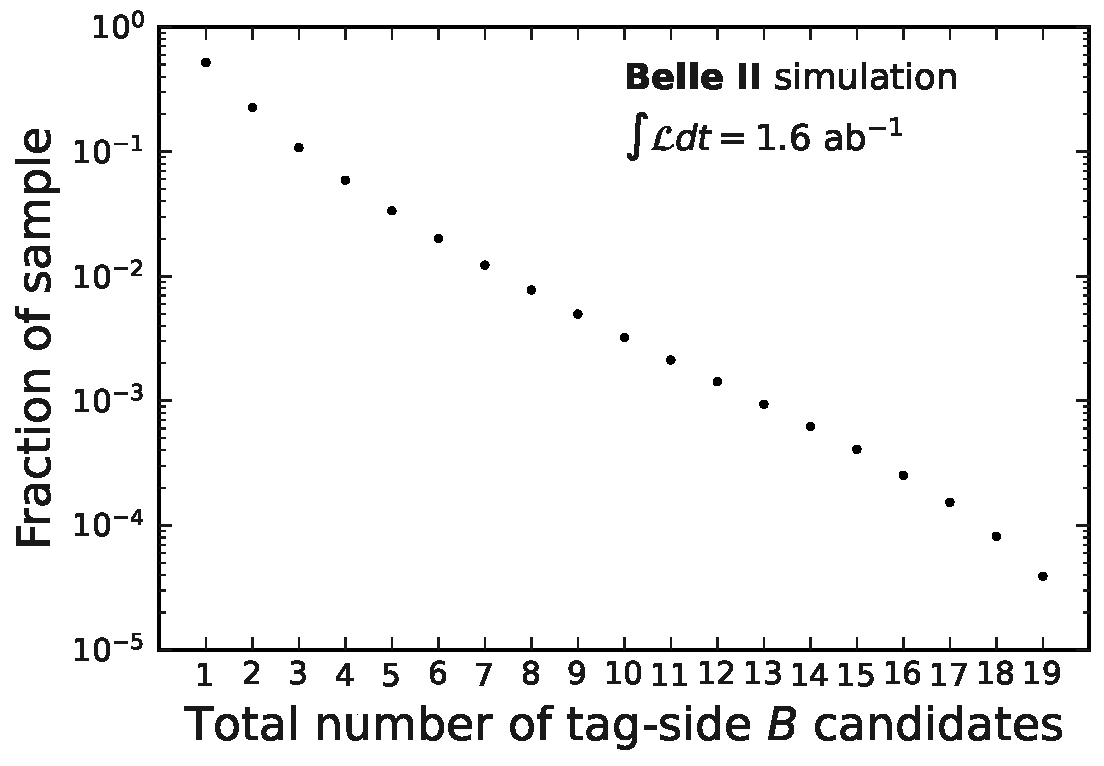
\includegraphics[width=0.45\textwidth]{figures/event_reconstruction/Bp_total_tag_candidates.pdf}
        }
    \subcaptionbox{\label{fig:fei_tag_reco_candidates_bzero}}{
    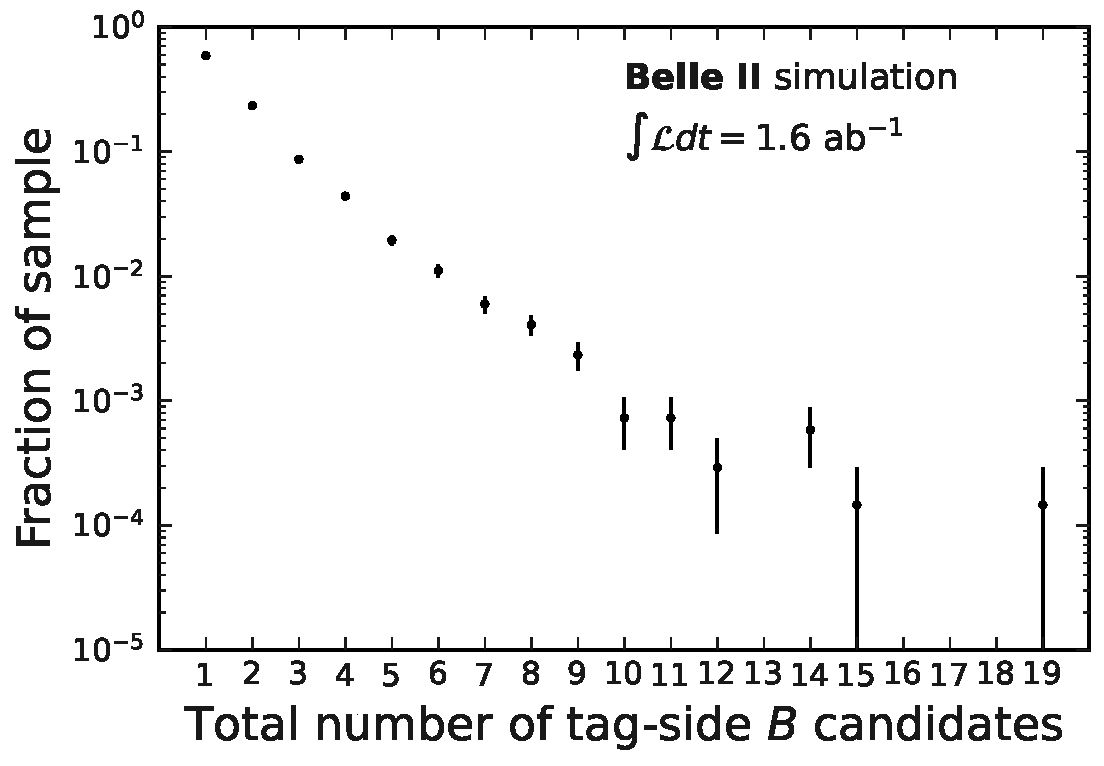
\includegraphics[width=0.45\textwidth]{figures/event_reconstruction/Bz_total_tag_candidates.pdf}
    }
    \caption{\label{fig:fei_tag_reco_candidates} Relative fractions of events for the number of reconstructed \B meson candidates.
    }
\end{figure}



% \subsection{Event topology reconstrunction}
% Many quantities that parametrise the \epem collision product topology in terms of tracks and neutral clusters in the event will be used.
% Using a definition, equivalent to cleaned tracks and clusters we recon